\documentclass[12pt]{article}


%%% packages used %%%
\usepackage[T1]{fontenc}
\usepackage[utf8]{inputenc}
\usepackage{titlesec}
\usepackage{lastpage}
\usepackage{fancyhdr}
\usepackage{graphicx,wrapfig}
\usepackage{enumitem}
\usepackage{color,xcolor}
\usepackage[square,numbers,sort&compress]{natbib}
\usepackage{float}
\usepackage{morefloats}
\usepackage[section]{placeins}

%%% URL's and breaking them %%%
\usepackage{url}
\usepackage{breakurl} 
\usepackage[breaklinks]{hyperref}
\def\UrlBreaks{\do\/\do-}

%%% Good way to show TODO's %%%
\newcommand\todo[1]{\colorbox{yellow}{\textbf{TODO: #1}}}

%%% better references to figures %%%
\usepackage{cleveref} %must come after hyperref
\crefname{figure}{figure}{figure}


%%% language and hyphenation %%%
\usepackage[english]{babel}

%%% code windows %%%
\usepackage{listings}
\definecolor{dkgreen}{rgb}{0,0.6,0}
\definecolor{gray}{rgb}{0.5,0.5,0.5}
\definecolor{mauve}{rgb}{0.58,0,0.82}
\renewcommand{\lstlistingname}{Code}
\lstset{
	frame=tb,
	language=C,
	aboveskip=3mm,
	belowskip=3mm,
	showstringspaces=false,
	columns=fixed,
	basicstyle={\footnotesize\ttfamily},
	numbers=none,
	numberstyle=\tiny\color{gray},
	keywordstyle=\color{blue},
	commentstyle=\color{dkgreen},
	stringstyle=\color{mauve},
	breaklines=true,
	breakatwhitespace=true,
	tabsize=3,
	basewidth=.5em,
	captionpos=b
}

%%% header and footer %%%
\pagestyle{fancy}
\fancyfoot[R]{Page \thepage\ of \pageref{LastPage}}
\fancyfoot[C]{}
\fancyhead[R]{}
\fancyhead[L]{}

%%% formatting %%%
\newlength\tindent %no indent
\setlength{\tindent}{\parindent} %no indent
\setlength{\parindent}{0pt} %no indent
\renewcommand{\indent}{\hspace*{\tindent}} %no indent
\newcommand{\mylist}[2]{\vbox{\smallskip#1 \begin{enumerate}[topsep=3pt,itemsep=0pt,partopsep=1ex,parsep=1ex,label=$\bullet$] #2 \end{enumerate}}\bigskip} %my own listing format

%%% coloring and figures %%%
\definecolor{textgray}{RGB}{130,130,130}
\usepackage[font={color=textgray,small},figurename=Figure,labelfont={it,bf}]{caption} %for caption below images

%%% sections and references %%%
\newcommand*{\fullref}[1]{\hyperref[{#1}]{\autoref*{#1} \nameref*{#1}}} % One single link
\newcommand{\subsectionextra}[2][\medskip]{\bigskip\textbf{#2#1\newline}}


%%% Resize to normal a4paper and remove the rediculously large borders %%
\usepackage[a4paper,left=3cm, right=3cm, top=3.01cm, bottom=1.01cm]{geometry}
\setlength{\headheight}{1.1\baselineskip}

%%% Title and Author %%%
\newcommand{\thistitle}{Hazeu - Automatisch orchideeën inpakken Plan van Aanpak}
\author{}
\title{\thistitle}
\date{\today}
\newcommand{\version}{V0.1}
\fancyhead[C] {\color{textgray}\thistitle \space- \version\space - \today}
\def\headrule{\color{textgray}\rule{\textwidth}{.4pt}}


%%% Actual begin  %%%
\begin{document}
	\input{frontpage.tex}
	
	% !TeX spellcheck = nl_NL
\section{Achtergronden}

Hazeu Orchids is een teeltbedrijf dat zich sinds 2000 gespecialiseerd heeft op de teelt van de Phalaenopsis, oftewel Orchideeën.
Wekelijks leveren ze grote volumes hiervan aan de markt.

\bigskip

Bij verkoop van bepaalde bestellingen, worden op dit moment de bloemen handmatig in een doos geplaatst.
Dit kost veel tijd en mankracht.
Ook is het in de doos plaatsen van de bloemen zwaar op de rug.
Om deze redenen wil Hazeu dit proces automatiseren.
Hiervoor zijn transportbanden, een robotarm en een 3D machine-vision camera beschikbaar gemaakt.

\newpage

	\section{Opdracht}
	\textbf{Probleemstelling}
	Wanneer er bij het bedrijf Hazeu Orchids een order binnen komt voor verpakte orchideeën in dozen worden bij de productielijn een aantal werknemers geïnstalleerd. Deze werknemers plaatsen trays met orchideeën in kartonnen dozen welke vanaf een kar worden gepakt en in dozen worden geplaatst. Dit werk is eentonig en fysiek zwaar. Vooral de lage positie waarin de trays in de doos worden gepaaltst is ergonomisch slecht.
	\vspace{5mm}
	
	\textbf{Opdracht omschrijving}
	Het ontwerpen van robot oplossing welke twee gevulde normpack  206, 208 of 209 trays, vanaf lopende transportband, kan verplaatsen in een doos van 60x40x80 cm. Deze dozen zijn vooraf gevouwen en op een transportbaan geplaatst. De dozen worden bij et plaatsen van de trays stilgezet. Bij deze handeling mogen de planten niet worden beschadigd en de doorlooptijd is maximaal 15 seconden per tray.
	
	
\newpage

	\section{Projectresultaten}
Het project kan worden opgedeeld in meerdere fases. Bij iedere fase zijn bijbehorende documenten welke moet worden opgeleverd om naar de volgende fase te gaan. \\[0.5cm]

\textbf{Initialisatiefase}


\begin{itemize}
	\item Samenwerkingsovereenkomst
	\begin{itemize}
		\item Ondertekend samenwerkingsovereenkomst
	\end{itemize}
	\item Plan van aanpak
	\begin{itemize}
		\item Hierin staat vastgesteld hoe, wat en waar de taken worden uitgevoerd de komende projectweken
		\item Organisatie
		\item I/O diagram
		\item Product breakdown structure
		\item Return of investment
		\item Kosten baten
	\end{itemize}
\end{itemize}


\textbf{Definitiefase}
Het pakket van eisen wordt gecontroleerd op volledigheid en doorgenomen met de klant of bepaald of het einddoel ongewijzigd is. 

\begin{itemize}
	\item Programma van eisen
	\begin{itemize}
		\item Een gesprek met de opdrachtgever om duidelijkheid te krijgen over diverse minimale eisen
		\item Een eisenpakket samengesteld uit eisen en wensen van de opdrachtgever
	\end{itemize}
	\item Testplan
\end{itemize}

\textbf{Voorbereidingsfase}
Het project wordt vervolgt vanaf de voorbereidingsfase. Hier het ontwerp uitgewerkt. Producten aan het einde van deze fase zijn:\\
\begin{itemize}
	\item Elektrisch ontwerp
	\begin{itemize}
		\item 3D wiring diagram
		\item Wiring diagram
		\item Componentenlijst
	\end{itemize}
	\item Mechanisch ontwerp (3D CAD live walk-through)
	\item Pneumatisch ontwerp
	\item Vision algoritme
\end{itemize}

\textbf{Realisatiefase} 
In de realisatiefase wordt het prototype geproduceerd. Daarbij behorende producten zijn:
\begin{itemize}
	\item Webartikel
	\item Film
	\item Prototype
	\item Technische documentatie
\end{itemize}
\newpage

	
	\section*{PBS}

Onderstaand is het PBS van het planten inpak systeem. Het product wordt onderverdeeld in de verschillende onderdelen.

\begin{enumerate}[label*=\arabic*.]
	\item Robot systeem
	\begin{enumerate}[label*=\arabic*.]
		\item Robot keuze
		\item Robot code
		\begin{enumerate}[label*=\arabic*.]
			\item Oppak code
			\item Neerzet code
		\end{enumerate}
	\end{enumerate}
	\item EOAT
	\begin{enumerate}[label*=\arabic*.]
		\item Hardware
		\begin{enumerate}[label*=\arabic*.]
			\item Concept generatie
			\item Concept keuze
			\item Prototype
		\end{enumerate}
		\item Code
	\end{enumerate}
	\item Vision systeem
	\begin{enumerate}[label*=\arabic*.]
		\item Tray detectie
		\begin{enumerate}[label*=\arabic*.]
			\item Camera systeem
			\begin{enumerate}[label*=\arabic*.]
				\item Keuze camera
				\item Keuze software
				\item Code
			\end{enumerate}
			\item Lichtsysteem
		\end{enumerate}
		\item Doos detectie
			\begin{enumerate}[label*=\arabic*.]
				\item Camera systeem
				\begin{enumerate}[label*=\arabic*.]
					\item Keuze camera
					\item Keuze software
					\item Code
				\end{enumerate}
				\item Lichtsysteem
			\end{enumerate}
		\end{enumerate}
	\item Control systeem
	\begin{enumerate}[label*=\arabic*.]
		\item HMI systeem
		\begin{enumerate}[label*=\arabic*.]
			\item Keuze HTML
			\item Interface
		\end{enumerate}
		\item PLC
		\begin{enumerate}[label*=\arabic*.]
			\item Keuze PLC
			\item Software
			\item Hardware
		\end{enumerate}
	\end{enumerate}
\end{enumerate}

\newpage

\begin{landscape}
	\begin{figure}[h]
		\centering
		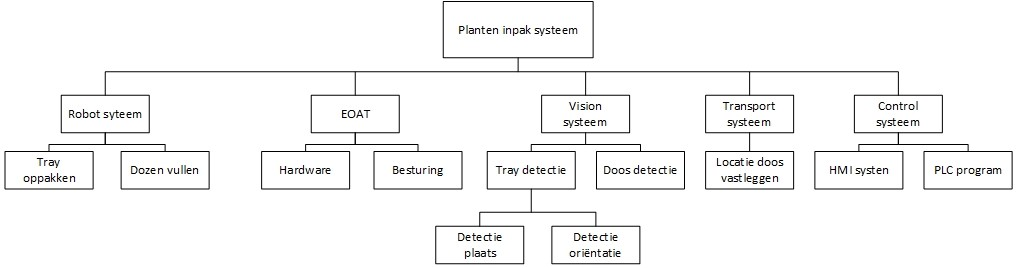
\includegraphics[scale=0.5]{Afbeeldingen/PBS.jpg}
		\caption{PBS} 
	\end{figure}
\end{landscape}

\newpage

	
	% !TeX spellcheck = nl_NL
\section{Kwaliteit}

%veiligheidsnormen
%referenties invoegen
Om de kwaliteit van Orchidee-inpaksysteem te waarborgen, wordt ROS-industrial gebruikt voor de robotaansturing.
Voor het vision algoritme wordt het open source OpenCV pakket gebruikt.
Zowel de aansturing van de robotarm als het vision algoritme wordt in C++ geïmplementeerd.
Voordat er code wordt geschreven, worden er ontwerpen gemaakt in UML \cite{UML}.
Deze ontwerpen worden vervolgens geïmplementeerd conform de clean code principes \cite{CLEAN_CODE}.

Het robotsysteem inclusief de End-Of-Arm-Tool zal voldoen aan de eisen voor een CE keurmerk volgens de Machinerichtlijn \cite{Machinerichtlijn}.

\newpage
	
	\section{Return on Investment}

	
	%%% the references made by bib (see citation.bib) %%%
	\bibliographystyle{unsrtnat}
	\renewcommand\bibsection{\section*{Literature and references}}
	\addcontentsline{toc}{section}{\protect Literature and references}%
	\bibliography{citations}
	
	
\end{document}